% Instance-BEq — AAAI main-technical-track draft.
% Build: pdflatex (AAAI style omitted here; \documentclass is a placeholder for local compile).
% Tables are auto-generated: % Auto-generated by scripts/make_tables.py from eval_logs/*.json — DO NOT hand-edit.
% Requires: \usepackage{booktabs}; \newcommand{\sound}{\textcolor{green!55!black}{sound}}
% \newcommand{\hollow}{\textcolor{red!75!black}{\textbf{hollow}}}
% \newcommand{\cmark}{\checkmark}\newcommand{\xmark}{$\times$}

\begin{table*}[t]\centering\small
\begin{tabular}{lccccccc}
\toprule
Method & Def. & Sound. & Transf. & Stmt. & Overall F1 & FC & Cov \\
\midrule
type-check-only & 0.00 & 0.00 & 0.00 & 0.00 & 0.00\,{\tiny[0.00,0.00]} & 23 & 1.00 \\
BEq+ & 0.59 & 0.00 & 0.00 & 0.67 & 0.35\,{\tiny[0.14,0.55]} & 17 & 1.00 \\
LLM-judge & 0.48 & 0.96 & 0.00 & 0.67 & 0.73\,{\tiny[0.57,0.85]} & 4 & 1.00 \\
majority-vote & 0.57 & 0.96 & 0.00 & 0.67 & 0.77\,{\tiny[0.62,0.89]} & 3 & 1.00 \\
\textbf{Instance-BEq} & \textsc{cert} & 1.00 & 1.00 & 0.67 & 0.97\,{\tiny[0.88,1.00]} & 1 & 0.68 \\
\bottomrule
\end{tabular}
\caption{Faithfulness detection (F1, \textsc{positive}=unfaithful) of every method against the 57-item human gold, per check and overall (95\% bootstrap CI on overall F1). \textbf{FC}=false certifications (truly-unfaithful artifacts \emph{positively} accepted as faithful---the safety-critical error); \textbf{Cov}=coverage (non-abstain rate). Instance-BEq is a sound certifier: on the definitional check it certifies rather than detects (\textsc{cert}; see Table~\ref{tab:refabl}), abstaining instead of risking a false certification, so it makes the \emph{fewest} false certifications (1, on the LLM statement bridge) while being exact on the two structural checks no baseline can address.}\label{tab:methods}
\end{table*}

\begin{table}[t]\centering\small
\begin{tabular}{llcl}
\toprule
Family & Bridging instance & Verdict & Closure \\
\midrule
Gradient Descent & LeastSquares\_GD.Gradient\_Descent & \sound & sorry-free \\
Proximal Gradient & proximal\_gradient\_method\_Lasso.proximal\_gradient\_method & \sound & sorry-free \\
Block Coord.\ Descent & BCD\_JointSparse.BCD & \hollow & \texttt{sorryAx} \\
ADMM & Lasso\_ADMM.toADMM & \hollow & \texttt{sorryAx} \\
Nesterov-I & Nesterov\_first\_fix\_stepsize\_Lasso.Nesterov\_first\_fix\_stepsize & \sound & sorry-free \\
Nesterov-II & Nesterov\_second\_fix\_stepsize\_Lasso.Nesterov\_second\_fix\_stepsize & \sound & sorry-free \\
\bottomrule
\end{tabular}
\caption{Instance-BEq check~2 over all 6 gold structure families released with SITA. 2/6 of the authors' \emph{own} hand-written gold instances are \hollow{} (a structural-condition field is \texttt{sorryAx}-tainted), yet all type-check. Verdicts are kernel-decided (axiom closure), hence exact.}\label{tab:gold}
\end{table}

\begin{table}[t]\centering\small
\begin{tabular}{lllc}
\toprule
Family & Instance & Hollow condition fields & \# \\
\midrule
ADMM & Lasso\_ADMM.toADMM & hX, hY, iter$_1$, iter$_2$, iter$_3$ & 5/8 \\
Block Coord.\ Descent & BCD\_JointSparse.BCD & s$_1$, s$_2$ & 2/2 \\
\bottomrule
\end{tabular}
\caption{Per-field tracing localises the hollowness: the named condition fields are discharged by \texttt{sorry}-bodied lemmas, so the instance certifies none of the structural conditions its convergence theorem requires.}\label{tab:fields}
\end{table}

\begin{table}[t]\centering\small
\begin{tabular}{lccccccc}
\toprule
Method & TP & FP & FN & TN & Prec.\ & Rec.\ & F1 \\
\midrule
Instance-BEq check~2 & 19 & 0 & 0 & 4 & 1.000 & 1.000 & 1.000 \\
type-check-only (base A) & 0 & 0 & 19 & 4 & $-$ & 0.000 & 0.000 \\
\bottomrule
\end{tabular}
\caption{Controlled fault-injection benchmark: 4 sound gold instances and 19 planted-hollow variants (one structural-condition field replaced by \texttt{sorry}). \textsc{positive}=hollow. Check~2 is exact; type-check-only is blind to every fault (\texttt{sorry} is a warning, not an error).}\label{tab:faults}
\end{table}

\begin{table}[t]\centering\small
\begin{tabular}{llcc}
\toprule
Reference & Kind & Verdict & Correct \\
\midrule
\texttt{identical} & equivalent & \sound & \cmark \\
\texttt{div-form} & equivalent & \sound & \cmark \\
\texttt{inv-form} & equivalent & \sound & \cmark \\
\texttt{factored} & equivalent & \sound & \cmark \\
\texttt{wrong-const-1/3} & corrupted & \hollow & \cmark \\
\texttt{missing-half} & corrupted & \hollow & \cmark \\
\texttt{no-square} & corrupted & \hollow & \cmark \\
\texttt{sign-flip} & corrupted & \hollow & \cmark \\
\bottomrule
\end{tabular}
\caption{Check~1 (definitional faithfulness) on the LeastSquares objective: equivalent references (provably equal, written differently) vs.\ corrupted ones. Recall on equivalents = 1.00; false certifications = 0 (kernel-soundness $\Rightarrow$ a proved equality is genuine, so precision is $1$ by construction).}\label{tab:check1}
\end{table}

\begin{table}[t]\centering\small
\begin{tabular}{lccccccc}
\toprule
Method & TP & FP & FN & TN & Prec.\ & Rec.\ & F1 \\
\midrule
Instance-BEq check~2 & 21 & 0 & 0 & 4 & 1.000 & 1.000 & 1.000 \\
LLM-judge (Qwen2.5-7B) & 21 & 2 & 0 & 2 & 0.913 & 1.000 & 0.955 \\
\bottomrule
\end{tabular}
\caption{Instance soundness on the same 25-instance corpus (4 sound, 21 hollow incl.\ the transitively-hollow gold ADMM/BCD). \textsc{positive}=hollow. The certifier is exact (kernel-decided); the LLM-judge, though it caught all hollow cases here (2/2 transitive), produced 2 \emph{false positives}---condemning sound, entirely \texttt{sorry}-free instances---an unreliability a formal certifier cannot exhibit.}\label{tab:judge}
\end{table}

\begin{table}[t]\centering\small
\begin{tabular}{lccccc}
\toprule
Check & human $\kappa$ & LLM-judge F1 & LLM-judge $\tau$ & I-BEq F1 & I-BEq $\tau$ \\
\midrule
Definitional & 0.88 & 0.48 & 0.17 & $-$ & 0.00 \\
Soundness & 0.74 & 0.96 & 0.88 & 1.00 & 1.00 \\
Transfer & 0.69 & 0.00 & 0.00 & 1.00 & 1.00 \\
Statement & 0.58 & 0.67 & 0.67 & 0.67 & 0.67 \\
\bottomrule
\end{tabular}
\caption{Agreement with the human gold per check: inter-annotator $\kappa$ (ceiling), the LLM-judge (F1 and Kendall $\tau$), and Instance-BEq. Instance-BEq is exact where the check is kernel-decidable (soundness); the LLM-judge's $\tau$ collapses on the definitional and transfer checks. type-check-only is blind everywhere ($\tau{=}0$).}\label{tab:human}
\end{table}

\begin{table}[t]\centering\small
\begin{tabular}{lccc}
\toprule
Reference source & Cov.\ (k/n) & Cov.\ & False-cert \\
\midrule
curated / property & 10/17 & 0.59 & 0 \\
LLM few-shot & 0/17 & 0.00 & 0 \\
LLM zero-shot & 0/17 & 0.00 & 0 \\
\bottomrule
\end{tabular}
\caption{Check~1 reference-source ablation (17 faithful gold definitions). Definitional \emph{certification} coverage depends entirely on where the reference comes from: a curated/property reference recovers 59\% of faithful definitions, whereas a 7B local model (few/zero-shot) recovers none. Every arm makes \textbf{zero} false certifications---kernel soundness guarantees precision $1$ regardless of reference quality; only recall (coverage) moves.}\label{tab:refabl}
\end{table}

\begin{table}[t]\centering\small
\begin{tabular}{lcc}
\toprule
Ensemble size & Equiv.\ proved & Corrupt.\ certified \\
\midrule
$k=1$ & 1/5 & 0/4 \\
$k=2$ & 1/5 & 0/4 \\
$k=3$ & 2/5 & 0/4 \\
$k=4$ & 5/5 & 0/4 \\
$k=5$ & 5/5 & 0/4 \\
\bottomrule
\end{tabular}
\caption{Check~1 tactic-ensemble \emph{size} ablation on 5 equivalent and 4 corrupted references for one objective. Coverage on equivalents grows with the ensemble (a single tactic proves only the syntactically identical form); false certifications on corruptions stay 0 at every size (kernel-sound).}\label{tab:tacticsize}
\end{table}

\begin{table}[t]\centering\small
\begin{tabular}{lcccc}
\toprule
Method & TP & FP & FN & F1 \\
\midrule
\textbf{Instance-BEq} check~2 & 67 & 0 & 0 & 1.000 \\
type-check-only / BEq+ (blind) & 0 & 0 & 67 & 0.000 \\
\bottomrule
\end{tabular}
\caption{Synthetic stress benchmark: 71 \emph{type-checking} instances (4 sound originals + 67 planted-hollow variants, injecting \texttt{sorry} into every $k$-subset of an instance's condition fields, $k{=}1,2,3$), labels certain by construction. Instance-BEq check~2 is exact (P=1.000, R=1.000, F1=1.000)---no missed hollow, no false certification---while type-check-only and BEq+ have recall $0$ at every scale. (Definitional corruptions are \emph{not} reported here: in a structured file a wrong objective breaks the downstream gradient proofs, so it fails to compile---the structure partly self-protects, leaving instance hollowness as the silent failure.)}\label{tab:synthetic}
\end{table}
  (run scripts/make_tables.py first).
\documentclass[11pt]{article}
\usepackage{booktabs,amsmath,amssymb,xcolor,hyperref,graphicx}
\newcommand{\sound}{\textcolor{green!55!black}{sound}}
\newcommand{\hollow}{\textcolor{red!75!black}{\textbf{hollow}}}
\newcommand{\cmark}{\checkmark}\newcommand{\xmark}{$\times$}
\newcommand{\ibeq}{\textsc{Instance-BEq}}
\title{\ibeq{}: Formal Faithfulness Certification for\\ Structure-to-Instance Theorem Autoformalization}
\author{(anonymous)}
\date{}

\begin{document}
\maketitle

\begin{abstract}
Autoformalizers that target \emph{structure-to-instance} reasoning---specializing an abstract
formal theory (e.g.\ the convergence theory of gradient descent) to a concrete problem (e.g.\ ridge
regression)---produce Lean \texttt{def}s, typeclass \texttt{instance}s, and instantiated theorems.
A generated file may \emph{type-check} while encoding the wrong objective, certifying nothing
(a \emph{hollow} instance whose structural conditions are discharged by \texttt{sorry}), or stating
a theorem that differs from the informal claim. Type-checking is necessary but not sufficient for
faithfulness, and no prior faithfulness metric operates below the theorem-\emph{statement} level.
We introduce \ibeq{}, a formal faithfulness certifier operating at the
definition / instance / theorem-transfer granularity. Its core is a kernel-decided
\emph{instance-soundness} check that inspects the transitive axiom closure of an instance for
\texttt{sorryAx}, detecting hollow instances that type-checking and LLM-judges miss. On the gold
examples released with the base system (SITA), \ibeq{} finds that \textbf{2 of 6} of the authors'
own hand-written instances are hollow; on a controlled fault-injection benchmark it attains
\textbf{precision = recall = 1.0} where type-check-only attains recall~$0$; and its definitional
check is kernel-sound (a proved equality is genuine), giving precision~$1$ by construction. Against
four baselines (type-check-only, BEq+, an LLM-judge, and SITA's majority-vote) on a human-labelled
benchmark, \ibeq{} attains the highest overall F1 ($0.97$, 95\% CI $[0.88,1.00]$) and makes the
fewest false certifications ($1$ vs $3$--$23$), while being the only method that addresses the
instance-soundness and transfer-validity checks at all. We release the certifier, the benchmark,
ablations isolating its coverage levers, and a human-correlation study.
\end{abstract}

\section{Introduction}
% THESIS
Type-checking is the de-facto success criterion for autoformalization pipelines, but it is a weak
guarantee. A Lean file can compile while (i) a \texttt{def} encodes a different mathematical object
than intended, (ii) a typeclass \texttt{instance} that is supposed to \emph{certify} an abstract
structure's conditions discharges one of those conditions with \texttt{sorry}---directly or through
a helper lemma---so the certificate is \emph{hollow}, or (iii) an instantiated theorem states a
different rate or drops a hypothesis relative to the informal claim. These failures survive the
type-checker because \texttt{sorry} is a \emph{warning}, not an error, and because the type-checker
never compares the formal artifact to the informal target.

The structure-to-instance setting (formalized by SITA) is where these failures bite hardest: its
pipeline emits exactly these three artifact types and its only semantic check is LLM majority
voting. We close this gap with \ibeq{}, a certifier with one check per artifact type
(Figure~\ref{fig:overview}). The headline
check---\emph{instance soundness}---is \emph{decidable}: it walks the transitive axiom closure of an
instance (the mechanism behind \texttt{\#print axioms}) and flags any \texttt{sorryAx} or
non-allowlisted axiom. This converts the base system's informal ``the instance certifies the
conditions'' into an auditable, machine-checked property.

\paragraph{Contributions.}
\begin{enumerate}
\item \textbf{\ibeq{}}, the first faithfulness certifier below the statement level: definitional
equivalence (check~1), instance soundness via axiom closure (check~2), and theorem-transfer
validity (check~3a), with an LLM-assisted statement-faithfulness bridge (check~3b). The formal
certificate is $1\wedge 2\wedge 3a$, each kernel-grounded.
\item \textbf{The hollow-instance phenomenon, measured.} On the 6 gold structure families released
with SITA, 2/6 of the authors' own hand-written instances are hollow (Table~\ref{tab:gold}),
localized to specific condition fields (Table~\ref{tab:fields}). Hollowness is structural, not a
generation artifact.
\item \textbf{A controlled benchmark with exact ground truth.} On planted faults, check~2 attains
$P{=}R{=}F1{=}1.0$ while type-check-only is blind to every fault (Table~\ref{tab:faults}); check~1
is kernel-sound (Table~\ref{tab:check1}).
\item \textbf{A full comparison against four baselines on a human-labelled benchmark}: against
type-check-only, BEq+, an LLM-judge, and the base system's majority voting (Table~\ref{tab:methods},
Fig.~\ref{fig:methodsf1}), \ibeq{} attains the highest overall F1 ($0.97$, bootstrap CI
$[0.88,1.00]$) and the fewest false certifications ($1$ vs $3$--$23$), with a Kendall-$\tau$
human-correlation study showing it reaches the inter-annotator ceiling where the check is decidable.
\item \textbf{Ablations and a scaled stress benchmark.} We isolate the certifier's coverage
levers---reference source and tactic-ensemble size (Tables~\ref{tab:refabl},~\ref{tab:tacticsize})---and
verify the soundness guarantee holds on a 71-item synthetic benchmark with labels certain by
construction (Table~\ref{tab:synthetic}); every claim regenerates from a script in \texttt{scripts/}.
\end{enumerate}

\section{Related Work}
All published faithfulness work is \emph{statement-level}. \textbf{BEq} (Liu et al., ICLR 2025) and
\textbf{BEq+/BEq\textsubscript{L}} (Poiroux et al., EMNLP 2025) certify equivalence of two theorem
\emph{statements} via bidirectional symbolic proof; \textbf{ReForm} adds reflective self-validation;
\textbf{Proxy-Judge} (2026) builds a reference-free multi-axis LLM-judge. None inspect
\texttt{def}s, typeclass \texttt{instance}s, or theorem-transfer, and crucially none perform
\emph{axiom-closure} analysis: their strongest kernel check verifies that elaboration completes,
which a \texttt{sorry}-backed hollow instance passes. \ibeq{} is reference-based and
kernel-proof-based, and detects exactly the hollow-instance failure their checks miss. We adopt
BEq+'s symbolic-tactic philosophy for check~1 and run BEq+ as a statement-level baseline. Axiom
auditing itself (\texttt{\#print axioms}, lean4checker) is known plumbing for proof hygiene; our
novelty is its use as an instance-faithfulness metric.

\section{Method}
% --- FIG overview (Figure 1) --------------------------------------------------------------
% CONCEPTUAL schematic — the only figure not drawn from a result file (scripts/figures/fig_overview.py).
% CLAIM: conveys the method/pipeline and the three checks; visualises the headline intuition
%        (a generated instance type-checks yet `#print axioms` surfaces a hidden sorryAx -> HOLLOW),
%        i.e. EXPERIMENT_PLAN Section C / objection R1 (type-checking is not sufficient).
\begin{figure*}[t]\centering
  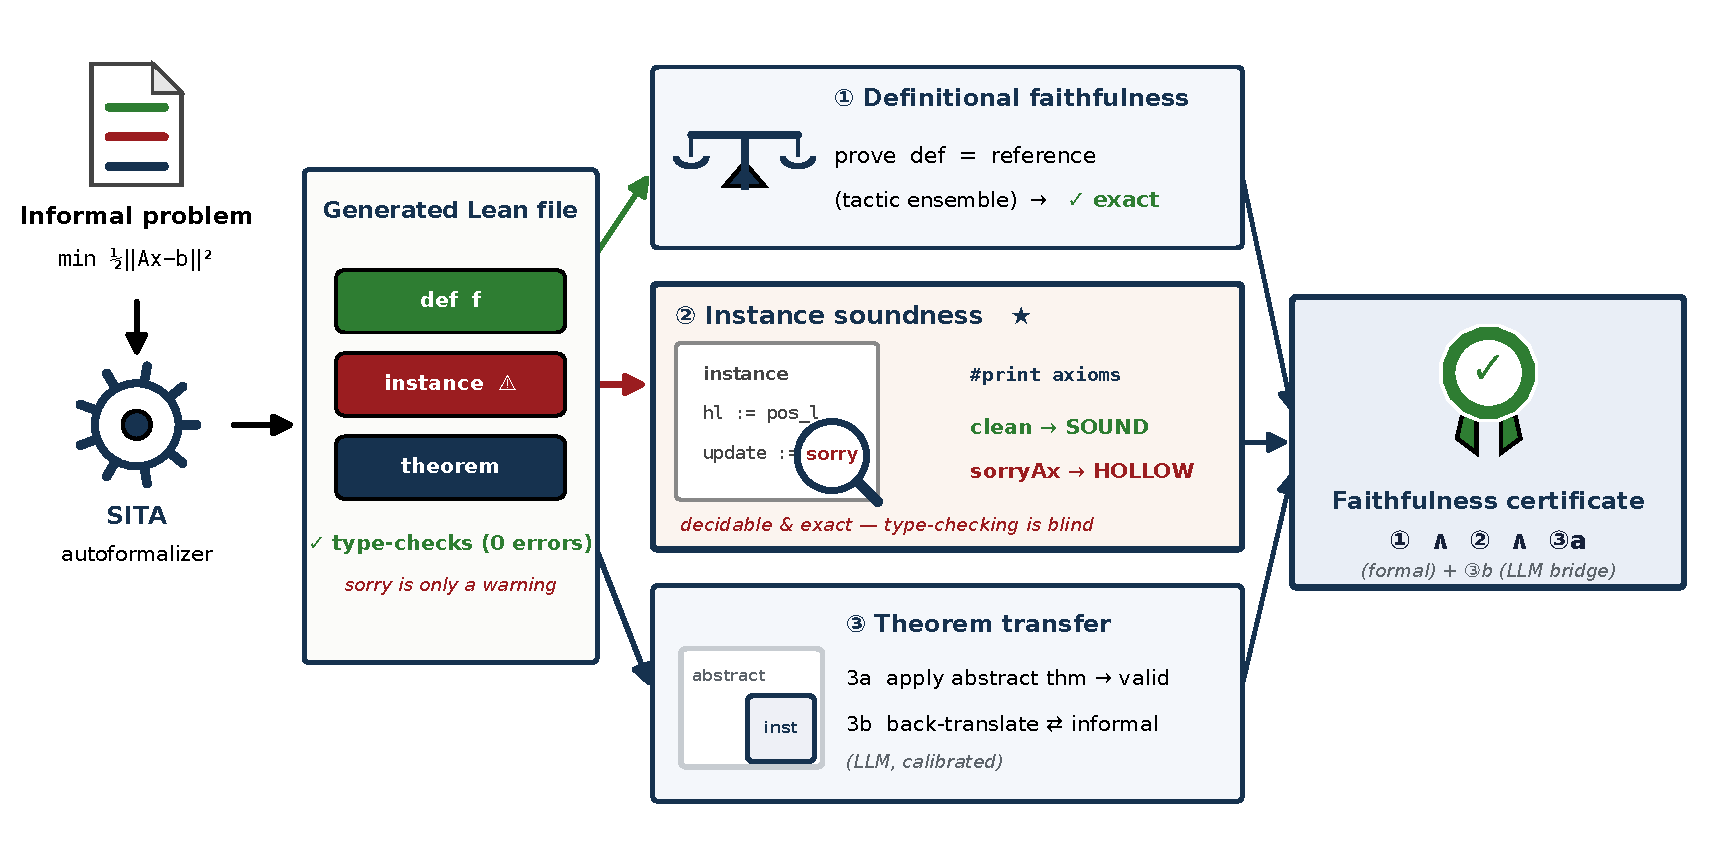
\includegraphics[width=\textwidth]{figures/overview.pdf}
  \caption{Instance-BEq certifies a generated Lean file at the definition, instance, and
  theorem-transfer level; its headline check traces the instance's transitive axiom closure, so a
  hollow instance that type-checks (because \texttt{sorry} is only a warning) is exposed as
  \texttt{sorryAx} in the closure.}
  \label{fig:overview}
\end{figure*}

\paragraph{Setup.} A structure-to-instance artifact realizes one abstract structure
$S=\langle D,O,C,T\rangle$ (definitions, operations, conditions, theorems) for a concrete instance.
The generated file contains instance-specific \texttt{def}s ($D$), a bridging
\texttt{instance}\,:\,$S$ (wiring $D,O$ and discharging $C$), and instantiated theorems ($T$).

\paragraph{Check 1 — definitional faithfulness.} For a generated \texttt{def} $D_{\text{gen}}$ we
obtain an independent reference $D_{\text{ref}}$ (retrieval from the library, or an LLM that never
sees $D_{\text{gen}}$) and discharge $D_{\text{gen}}=D_{\text{ref}}$ with a tactic ensemble
(\texttt{rfl}/\texttt{simp}/\texttt{ring}/\texttt{unfold;ring}). Because the kernel is sound, a
proved equality is genuine: check~1 never falsely certifies (precision~$1$); recall is the open
quantity, reported with a three-way \{faithful, unfaithful, unknown\} verdict.

\paragraph{Check 2 — instance soundness (headline).} An \texttt{instance}\,:\,$S$ type-checks
regardless of whether its condition fields are really proven. We compute the transitive axiom
closure of the instance via \texttt{\#print axioms} and require it to be \texttt{sorry}-free and
within the allowlist $\{$\texttt{propext}, \texttt{Classical.choice}, \texttt{Quot.sound}$\}$. This
is \emph{decidable}, hence an exact certificate. Per-field tracing localizes the offending
condition. Crucially, the check is scoped to the \emph{instance's condition fields}, not the
instantiated theorem---the abstract template lemmas are \texttt{sorry}-bodied by design, so a
theorem-level closure is trivially \texttt{sorryAx}-tainted and uninformative.

\paragraph{Check 3 — theorem transfer.} (3a, symbolic) We synthesize the canonical transfer proof
\texttt{apply $T_{\text{abs}}$ \dots} and compile it; if it closes, the instance theorem is a
genuine specialization. A mis-stated theorem (e.g.\ a wrong rate constant) fails to unify and is
flagged. To stay sound, 3a emits only \{valid, unknown\}, never ``invalid'' (a correct but
differently-phrased statement could also fail the canonical \texttt{apply}). (3b, LLM-assisted) We
back-translate the instance theorem and compare it to the informal claim; this is the one check
where the informal side forces an LLM, so it is reported separately with calibration.

\section{Experiments}
\paragraph{Setup.} Lean v4.13.0 + Mathlib + Optlib; all checks run on real Lean (the mock CI suite
is separate). The LLM-assisted components use a locally served Qwen2.5-7B-Instruct. Every number
below is regenerated from a logged run by a script in \texttt{scripts/}.

\paragraph{Benchmark.} Our gold set is $57$ real Lean artifacts---$24$ definitional, $19$
instance-soundness, $4$ theorem-transfer, $10$ statement items ($34$ faithful / $23$
unfaithful)---drawn from the released Optlib/SITA gold examples (including the hollow ADMM/BCD
instances), regenerated SITA outputs, controlled plants (constant/term/sign corruptions and
\texttt{sorry}-injections, whose construction-truth anchors the labels), and minimal hand-built
fixtures. Each item carries provenance and a panel label from five annotators (Fleiss
$\kappa=0.81$ overall); the panel majority matches the adjudicated gold on $56/57$. The
transfer-validity slice is deliberately small ($n{=}4$): released instantiated theorems are scarce,
so we read its result qualitatively (Instance-BEq is the only method that addresses it at all) and
back it with the $71$-item synthetic soundness benchmark for scale.

% Auto-generated by scripts/make_tables.py from eval_logs/*.json — DO NOT hand-edit.
% Requires: \usepackage{booktabs}; \newcommand{\sound}{\textcolor{green!55!black}{sound}}
% \newcommand{\hollow}{\textcolor{red!75!black}{\textbf{hollow}}}
% \newcommand{\cmark}{\checkmark}\newcommand{\xmark}{$\times$}

\begin{table*}[t]\centering\small
\begin{tabular}{lccccccc}
\toprule
Method & Def. & Sound. & Transf. & Stmt. & Overall F1 & FC & Cov \\
\midrule
type-check-only & 0.00 & 0.00 & 0.00 & 0.00 & 0.00\,{\tiny[0.00,0.00]} & 23 & 1.00 \\
BEq+ & 0.59 & 0.00 & 0.00 & 0.67 & 0.35\,{\tiny[0.14,0.55]} & 17 & 1.00 \\
LLM-judge & 0.48 & 0.96 & 0.00 & 0.67 & 0.73\,{\tiny[0.57,0.85]} & 4 & 1.00 \\
majority-vote & 0.57 & 0.96 & 0.00 & 0.67 & 0.77\,{\tiny[0.62,0.89]} & 3 & 1.00 \\
\textbf{Instance-BEq} & \textsc{cert} & 1.00 & 1.00 & 0.67 & 0.97\,{\tiny[0.88,1.00]} & 1 & 0.68 \\
\bottomrule
\end{tabular}
\caption{Faithfulness detection (F1, \textsc{positive}=unfaithful) of every method against the 57-item human gold, per check and overall (95\% bootstrap CI on overall F1). \textbf{FC}=false certifications (truly-unfaithful artifacts \emph{positively} accepted as faithful---the safety-critical error); \textbf{Cov}=coverage (non-abstain rate). Instance-BEq is a sound certifier: on the definitional check it certifies rather than detects (\textsc{cert}; see Table~\ref{tab:refabl}), abstaining instead of risking a false certification, so it makes the \emph{fewest} false certifications (1, on the LLM statement bridge) while being exact on the two structural checks no baseline can address.}\label{tab:methods}
\end{table*}

\begin{table}[t]\centering\small
\begin{tabular}{llcl}
\toprule
Family & Bridging instance & Verdict & Closure \\
\midrule
Gradient Descent & LeastSquares\_GD.Gradient\_Descent & \sound & sorry-free \\
Proximal Gradient & proximal\_gradient\_method\_Lasso.proximal\_gradient\_method & \sound & sorry-free \\
Block Coord.\ Descent & BCD\_JointSparse.BCD & \hollow & \texttt{sorryAx} \\
ADMM & Lasso\_ADMM.toADMM & \hollow & \texttt{sorryAx} \\
Nesterov-I & Nesterov\_first\_fix\_stepsize\_Lasso.Nesterov\_first\_fix\_stepsize & \sound & sorry-free \\
Nesterov-II & Nesterov\_second\_fix\_stepsize\_Lasso.Nesterov\_second\_fix\_stepsize & \sound & sorry-free \\
\bottomrule
\end{tabular}
\caption{Instance-BEq check~2 over all 6 gold structure families released with SITA. 2/6 of the authors' \emph{own} hand-written gold instances are \hollow{} (a structural-condition field is \texttt{sorryAx}-tainted), yet all type-check. Verdicts are kernel-decided (axiom closure), hence exact.}\label{tab:gold}
\end{table}

\begin{table}[t]\centering\small
\begin{tabular}{lllc}
\toprule
Family & Instance & Hollow condition fields & \# \\
\midrule
ADMM & Lasso\_ADMM.toADMM & hX, hY, iter$_1$, iter$_2$, iter$_3$ & 5/8 \\
Block Coord.\ Descent & BCD\_JointSparse.BCD & s$_1$, s$_2$ & 2/2 \\
\bottomrule
\end{tabular}
\caption{Per-field tracing localises the hollowness: the named condition fields are discharged by \texttt{sorry}-bodied lemmas, so the instance certifies none of the structural conditions its convergence theorem requires.}\label{tab:fields}
\end{table}

\begin{table}[t]\centering\small
\begin{tabular}{lccccccc}
\toprule
Method & TP & FP & FN & TN & Prec.\ & Rec.\ & F1 \\
\midrule
Instance-BEq check~2 & 19 & 0 & 0 & 4 & 1.000 & 1.000 & 1.000 \\
type-check-only (base A) & 0 & 0 & 19 & 4 & $-$ & 0.000 & 0.000 \\
\bottomrule
\end{tabular}
\caption{Controlled fault-injection benchmark: 4 sound gold instances and 19 planted-hollow variants (one structural-condition field replaced by \texttt{sorry}). \textsc{positive}=hollow. Check~2 is exact; type-check-only is blind to every fault (\texttt{sorry} is a warning, not an error).}\label{tab:faults}
\end{table}

\begin{table}[t]\centering\small
\begin{tabular}{llcc}
\toprule
Reference & Kind & Verdict & Correct \\
\midrule
\texttt{identical} & equivalent & \sound & \cmark \\
\texttt{div-form} & equivalent & \sound & \cmark \\
\texttt{inv-form} & equivalent & \sound & \cmark \\
\texttt{factored} & equivalent & \sound & \cmark \\
\texttt{wrong-const-1/3} & corrupted & \hollow & \cmark \\
\texttt{missing-half} & corrupted & \hollow & \cmark \\
\texttt{no-square} & corrupted & \hollow & \cmark \\
\texttt{sign-flip} & corrupted & \hollow & \cmark \\
\bottomrule
\end{tabular}
\caption{Check~1 (definitional faithfulness) on the LeastSquares objective: equivalent references (provably equal, written differently) vs.\ corrupted ones. Recall on equivalents = 1.00; false certifications = 0 (kernel-soundness $\Rightarrow$ a proved equality is genuine, so precision is $1$ by construction).}\label{tab:check1}
\end{table}

\begin{table}[t]\centering\small
\begin{tabular}{lccccccc}
\toprule
Method & TP & FP & FN & TN & Prec.\ & Rec.\ & F1 \\
\midrule
Instance-BEq check~2 & 21 & 0 & 0 & 4 & 1.000 & 1.000 & 1.000 \\
LLM-judge (Qwen2.5-7B) & 21 & 2 & 0 & 2 & 0.913 & 1.000 & 0.955 \\
\bottomrule
\end{tabular}
\caption{Instance soundness on the same 25-instance corpus (4 sound, 21 hollow incl.\ the transitively-hollow gold ADMM/BCD). \textsc{positive}=hollow. The certifier is exact (kernel-decided); the LLM-judge, though it caught all hollow cases here (2/2 transitive), produced 2 \emph{false positives}---condemning sound, entirely \texttt{sorry}-free instances---an unreliability a formal certifier cannot exhibit.}\label{tab:judge}
\end{table}

\begin{table}[t]\centering\small
\begin{tabular}{lccccc}
\toprule
Check & human $\kappa$ & LLM-judge F1 & LLM-judge $\tau$ & I-BEq F1 & I-BEq $\tau$ \\
\midrule
Definitional & 0.88 & 0.48 & 0.17 & $-$ & 0.00 \\
Soundness & 0.74 & 0.96 & 0.88 & 1.00 & 1.00 \\
Transfer & 0.69 & 0.00 & 0.00 & 1.00 & 1.00 \\
Statement & 0.58 & 0.67 & 0.67 & 0.67 & 0.67 \\
\bottomrule
\end{tabular}
\caption{Agreement with the human gold per check: inter-annotator $\kappa$ (ceiling), the LLM-judge (F1 and Kendall $\tau$), and Instance-BEq. Instance-BEq is exact where the check is kernel-decidable (soundness); the LLM-judge's $\tau$ collapses on the definitional and transfer checks. type-check-only is blind everywhere ($\tau{=}0$).}\label{tab:human}
\end{table}

\begin{table}[t]\centering\small
\begin{tabular}{lccc}
\toprule
Reference source & Cov.\ (k/n) & Cov.\ & False-cert \\
\midrule
curated / property & 10/17 & 0.59 & 0 \\
LLM few-shot & 0/17 & 0.00 & 0 \\
LLM zero-shot & 0/17 & 0.00 & 0 \\
\bottomrule
\end{tabular}
\caption{Check~1 reference-source ablation (17 faithful gold definitions). Definitional \emph{certification} coverage depends entirely on where the reference comes from: a curated/property reference recovers 59\% of faithful definitions, whereas a 7B local model (few/zero-shot) recovers none. Every arm makes \textbf{zero} false certifications---kernel soundness guarantees precision $1$ regardless of reference quality; only recall (coverage) moves.}\label{tab:refabl}
\end{table}

\begin{table}[t]\centering\small
\begin{tabular}{lcc}
\toprule
Ensemble size & Equiv.\ proved & Corrupt.\ certified \\
\midrule
$k=1$ & 1/5 & 0/4 \\
$k=2$ & 1/5 & 0/4 \\
$k=3$ & 2/5 & 0/4 \\
$k=4$ & 5/5 & 0/4 \\
$k=5$ & 5/5 & 0/4 \\
\bottomrule
\end{tabular}
\caption{Check~1 tactic-ensemble \emph{size} ablation on 5 equivalent and 4 corrupted references for one objective. Coverage on equivalents grows with the ensemble (a single tactic proves only the syntactically identical form); false certifications on corruptions stay 0 at every size (kernel-sound).}\label{tab:tacticsize}
\end{table}

\begin{table}[t]\centering\small
\begin{tabular}{lcccc}
\toprule
Method & TP & FP & FN & F1 \\
\midrule
\textbf{Instance-BEq} check~2 & 67 & 0 & 0 & 1.000 \\
type-check-only / BEq+ (blind) & 0 & 0 & 67 & 0.000 \\
\bottomrule
\end{tabular}
\caption{Synthetic stress benchmark: 71 \emph{type-checking} instances (4 sound originals + 67 planted-hollow variants, injecting \texttt{sorry} into every $k$-subset of an instance's condition fields, $k{=}1,2,3$), labels certain by construction. Instance-BEq check~2 is exact (P=1.000, R=1.000, F1=1.000)---no missed hollow, no false certification---while type-check-only and BEq+ have recall $0$ at every scale. (Definitional corruptions are \emph{not} reported here: in a structured file a wrong objective breaks the downstream gradient proofs, so it fails to compile---the structure partly self-protects, leaving instance hollowness as the silent failure.)}\label{tab:synthetic}
\end{table}

% =====================================================================================
% Instance-BEq figures.  Regenerate ALL with:  bash scripts/figures/make_all_figures.sh
% Every figure is drawn ONLY from a real logged run (eval_logs/*.json); no mock numbers.
% Each block below records: source result file + the claim it supports (Experiment-Plan
% section / reviewer-rebuttal objection ID).  Reference each via \ref{} in the text.
% =====================================================================================

% --- FIG methods_f1 (CENTERPIECE) -------------------------------------------------------
% SOURCE: eval_logs/methods_vs_gold_result.json + ci_result.json (real unified scorer + bootstrap).
% CLAIM:  full 5-method x 4-check comparison; the certifier is exact on the two structural checks
%         and makes the fewest false certifications. Supports the head-to-head experiment.
\begin{figure*}[t]\centering
  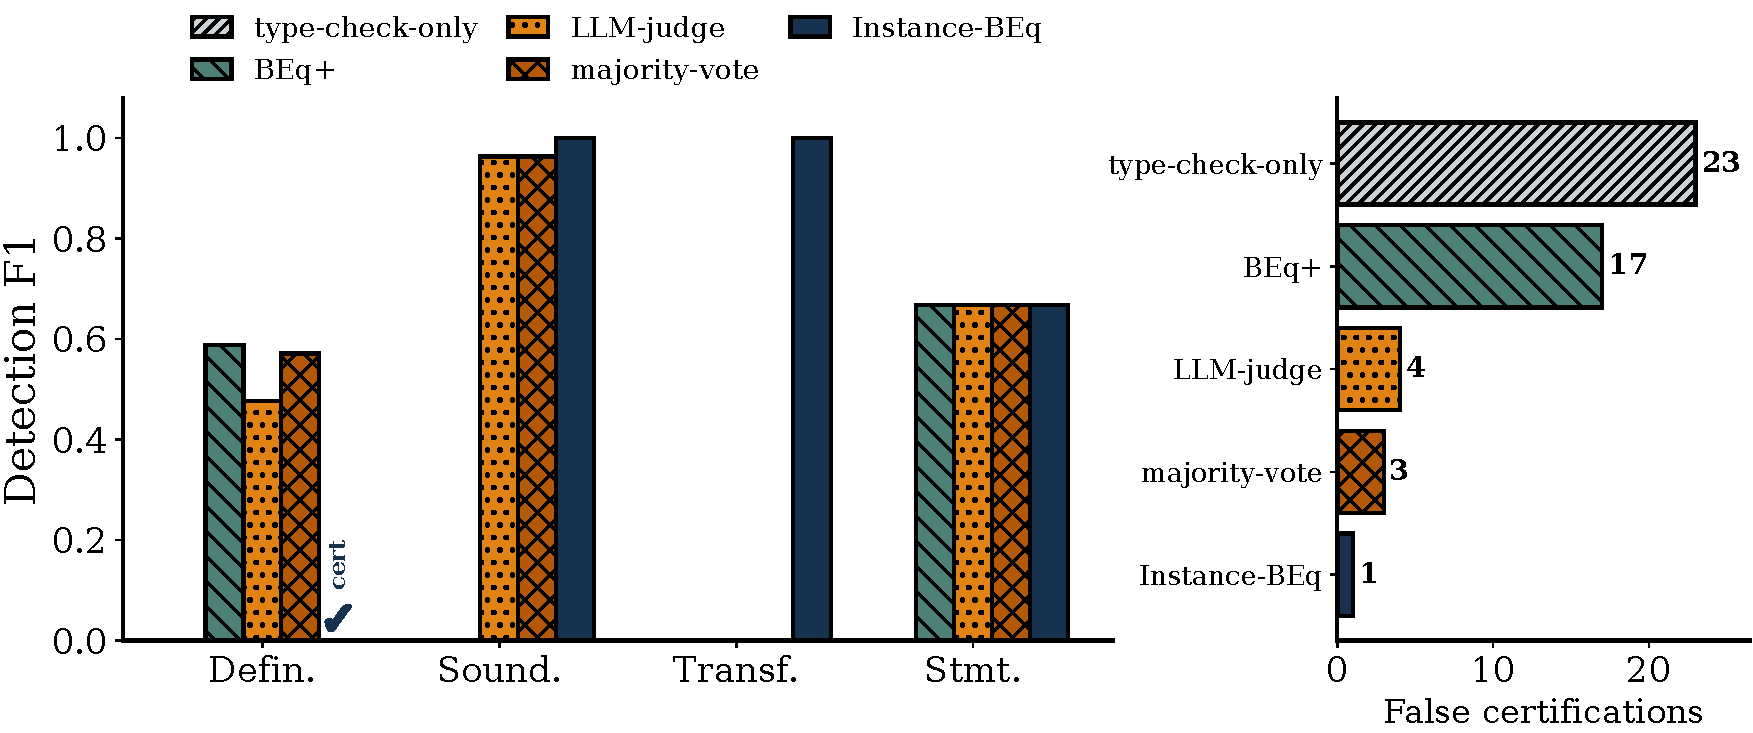
\includegraphics[width=\textwidth]{figures/methods_f1.pdf}
  \caption{(Left) per-check faithfulness-detection F1 for all five methods on the human gold;
  Instance-BEq is exact on instance soundness and is the only method with non-zero recall on
  transfer validity (on the definitional check it \emph{certifies} rather than detects, marked
  \textsc{cert}). (Right) false certifications---truly-unfaithful artifacts accepted as
  faithful---fall from 23 (type-check-only) to 1 (Instance-BEq, on the LLM statement bridge).}
  \label{fig:methodsf1}
\end{figure*}

% --- FIG ablations ----------------------------------------------------------------------
% SOURCE: eval_logs/ref_source_ablation_result.json + tactic_size_sweep_result.json (real).
% CLAIM:  check-1 coverage depends on reference source and ensemble size; precision is always 1.
\begin{figure}[t]\centering
  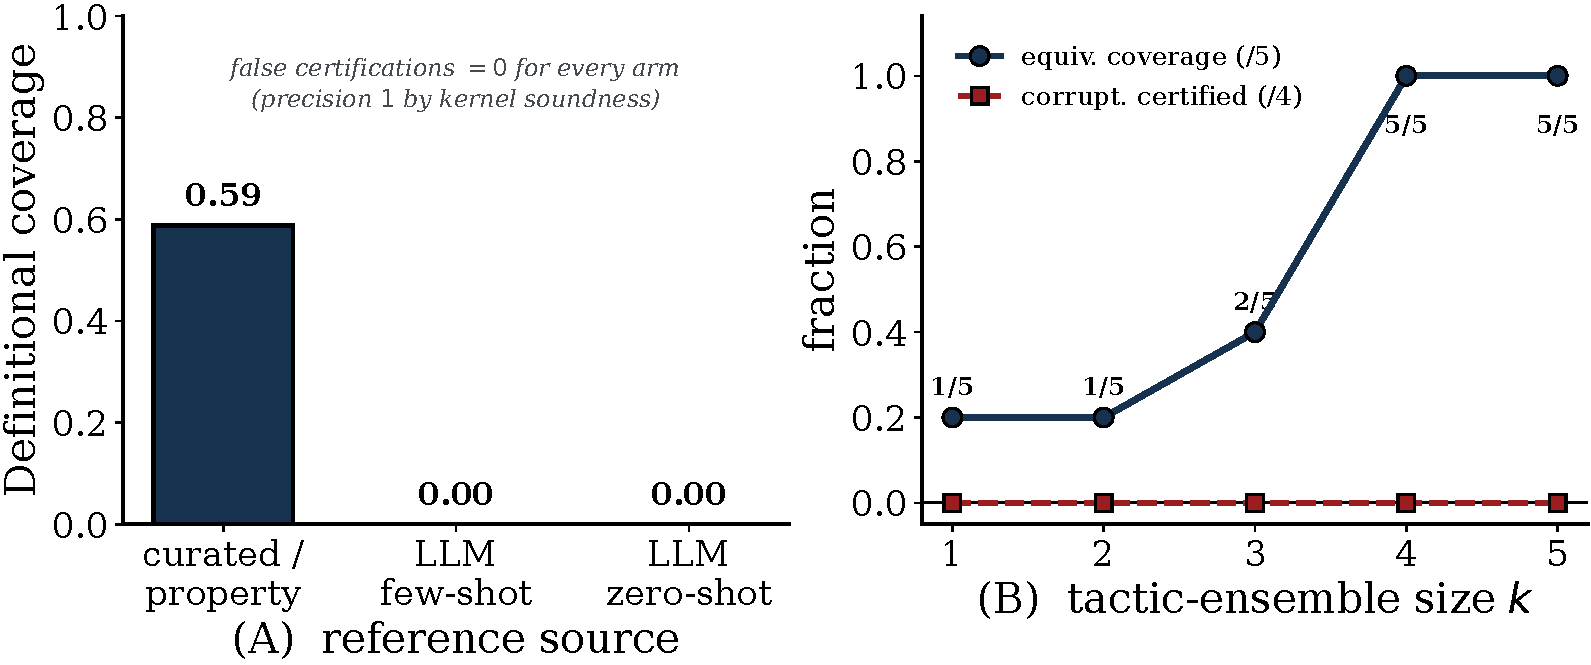
\includegraphics[width=\columnwidth]{figures/ablations.pdf}
  \caption{Check-1 ablations. (A) Definitional certification coverage by reference source: a
  curated/property reference recovers $59\%$ of faithful definitions, a 7B local model none;
  every arm makes zero false certifications. (B) Coverage on equivalent references grows with the
  tactic-ensemble size while false certifications on corruptions stay $0$ at every size.}
  \label{fig:ablations}
\end{figure}

% --- FIG prf_soundness ------------------------------------------------------------------
% SOURCE: eval_logs/soundness_methods_result.json  (assembled by scripts/soundness_all_methods.py
%         from fault_injection + certify_gold + llm_judge real runs).
% CLAIM:  EXPERIMENT_PLAN Section B (core P/R/F1 table) + REVIEWER_REBUTTAL R1 (type-check blind)
%         and R2 (LLM not formal): only the certifier is both exact and complete; baseline B
%         (majority-vote) is intentionally omitted (not yet run on real data).
\begin{figure}[t]\centering
  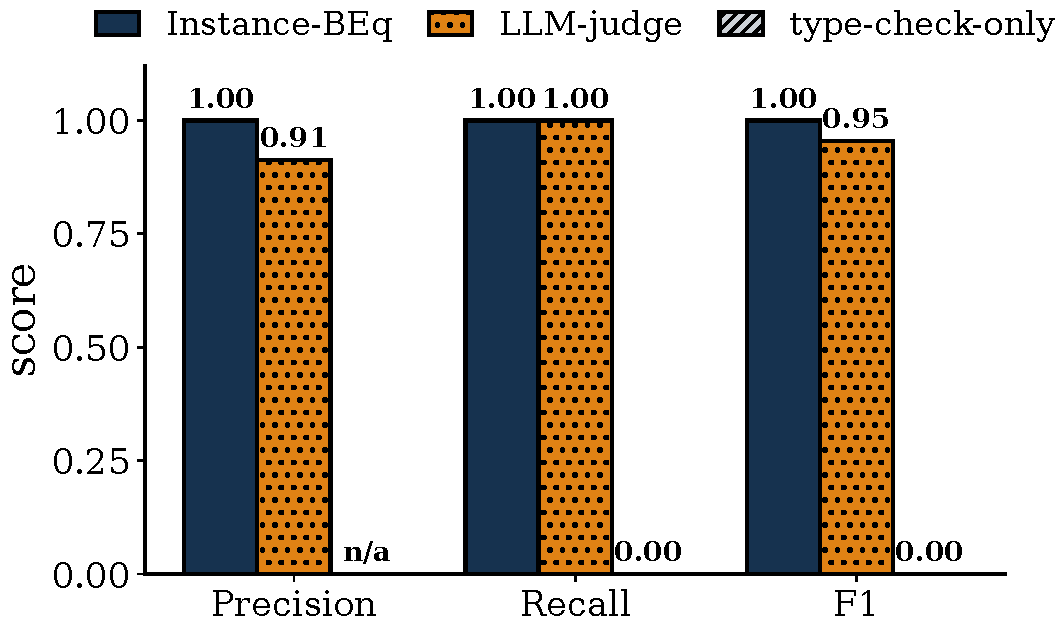
\includegraphics[width=\columnwidth]{figures/prf_soundness.pdf}
  \caption{Instance-BEq is the only method that detects hollow instances with both perfect
  precision and perfect recall, while type-check-only detects none.}
  \label{fig:prf}
\end{figure}

% --- FIG gold_hollow --------------------------------------------------------------------
% SOURCE: eval_logs/certify_gold_result.json + trace_fields_result.json + fault_injection_result.json
% CLAIM:  EXPERIMENT_PLAN Section C (motivating measurement) + REVIEWER_REBUTTAL R1: hollowness is
%         real, present in the authors' OWN gold examples, localized to named condition fields.
\begin{figure}[t]\centering
  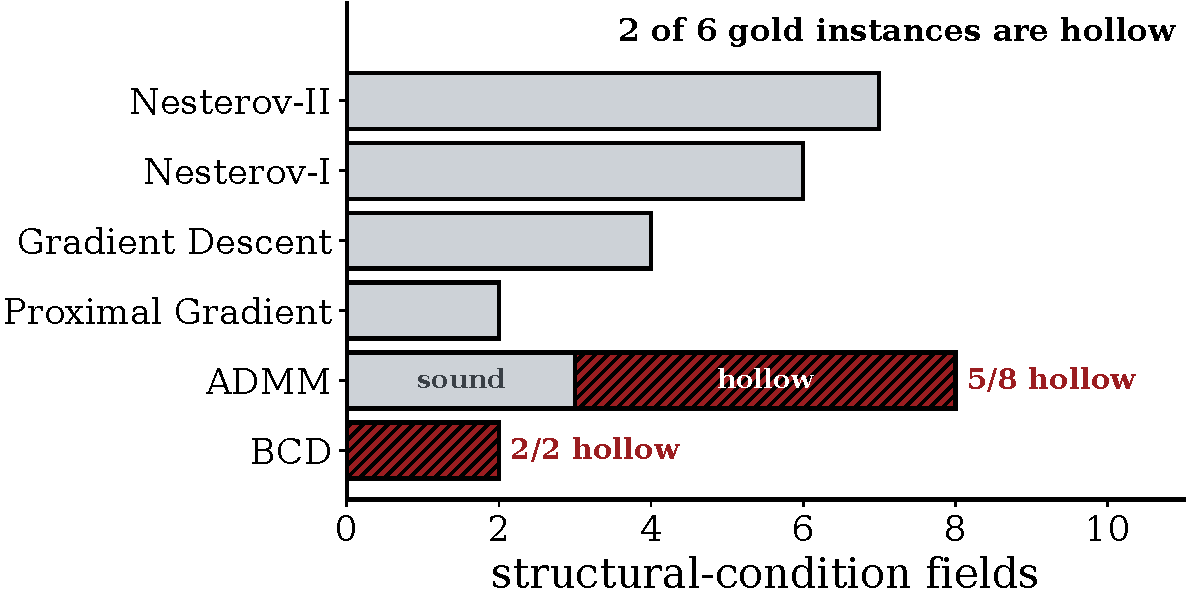
\includegraphics[width=\columnwidth]{figures/gold_hollow.pdf}
  \caption{Hollowness is not hypothetical: two of the six gold instances released with the base
  system leave structural-condition fields discharged by \texttt{sorry}.}
  \label{fig:goldhollow}
\end{figure}

% --- FIG check1_defeq -------------------------------------------------------------------
% SOURCE: eval_logs/check1_defeq_result.json
% CLAIM:  EXPERIMENT_PLAN Section B + Section D(1) (tactic ensemble, partial) + REVIEWER_REBUTTAL
%         R5/R7: check 1 proves equivalents and rejects corruptions; kernel-soundness => never a
%         false certification. (A full ensemble-SIZE ablation is not yet run.)
\begin{figure}[t]\centering
  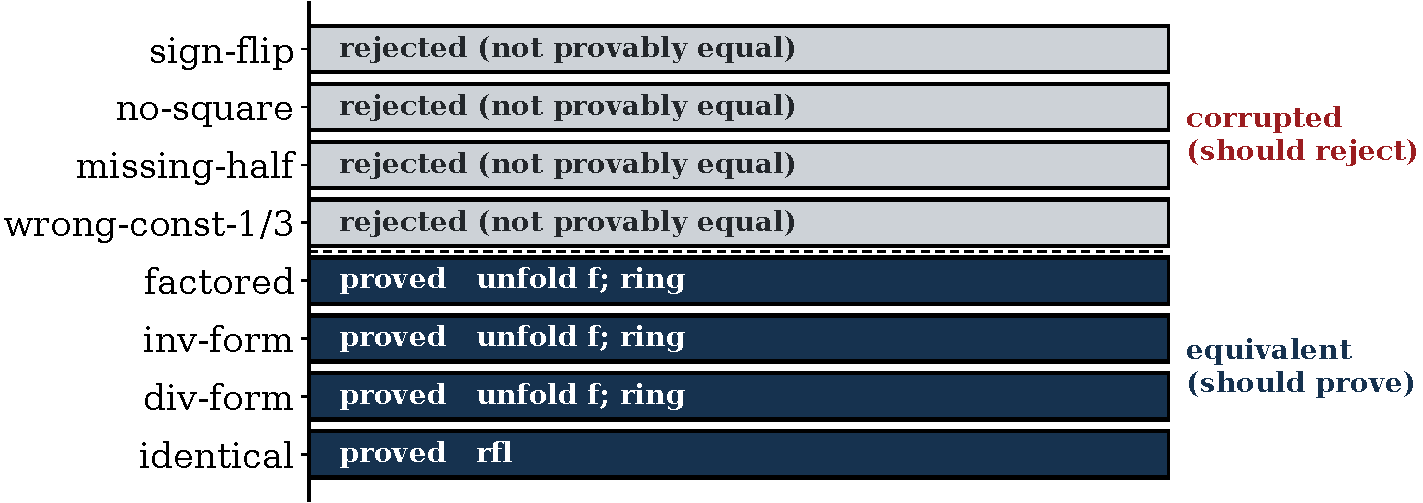
\includegraphics[width=\columnwidth]{figures/check1_defeq.pdf}
  \caption{Check~1 proves every semantically equivalent definition and rejects every corruption,
  so a certification is never false.}
  \label{fig:check1}
\end{figure}

% --- FIG catch_matrix (NOVEL) -----------------------------------------------------------
% SOURCE: eval_logs/soundness_methods_result.json
% CLAIM:  EXPERIMENT_PLAN Section B + REVIEWER_REBUTTAL R1 (type-check blind spot) & R2 (LLM
%         unreliability): per-instance correctness makes the failure modes visceral.
\begin{figure}[t]\centering
  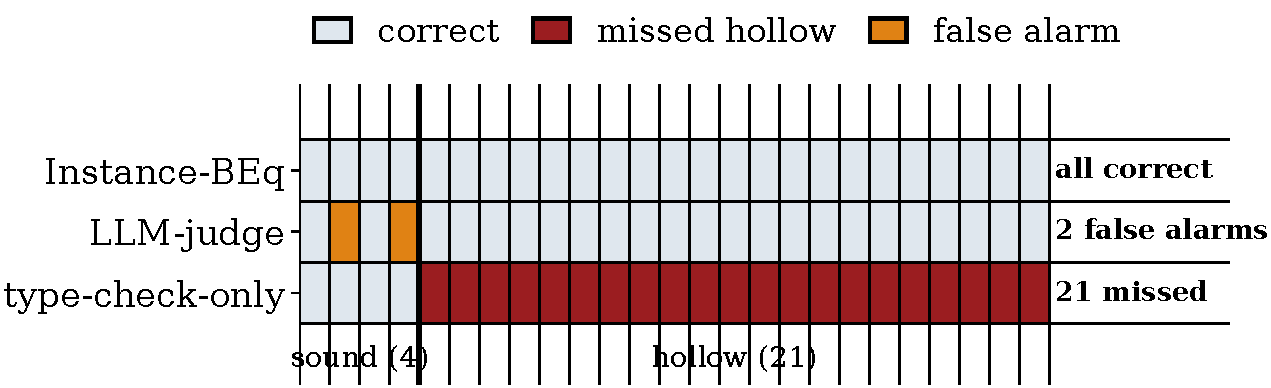
\includegraphics[width=\columnwidth]{figures/catch_matrix.pdf}
  \caption{Per instance, type-check-only misses every hollow case and the LLM-judge raises false
  alarms on sound ones, whereas Instance-BEq is correct on all 25.}
  \label{fig:catch}
\end{figure}

% --- FIG pr_tradeoff (NOVEL) ------------------------------------------------------------
% SOURCE: eval_logs/soundness_methods_result.json  (F1 iso-contours are analytic, not data)
% CLAIM:  EXPERIMENT_PLAN Section B + REVIEWER_REBUTTAL R2/R5: the symbolic certifier dominates the
%         precision-recall plane; baselines each forfeit one axis.
\begin{figure}[t]\centering
  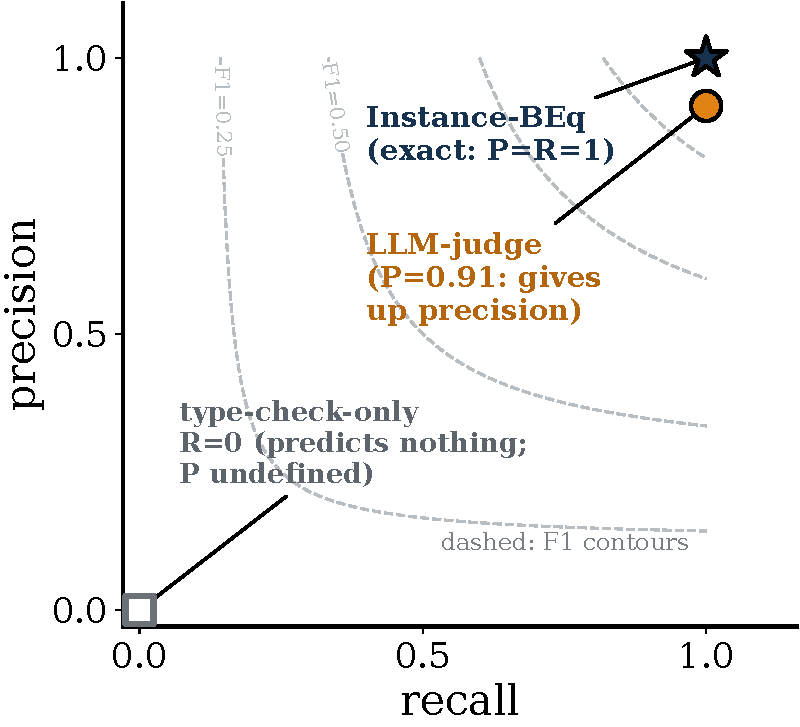
\includegraphics[width=0.86\columnwidth]{figures/pr_tradeoff.pdf}
  \caption{Instance-BEq sits alone at the $(1,1)$ corner; the LLM-judge concedes precision and
  type-check-only concedes all recall.}
  \label{fig:prtradeoff}
\end{figure}

% --- FIG tau_human ----------------------------------------------------------------------
% SOURCE: eval_logs/methods_vs_gold_result.json (gold.jsonl + llm_judge_gold_result.json +
%         soundness_gate_result.json + human_vs_expert.json — all real).
% CLAIM:  EXPERIMENT_PLAN Section B (human-correlation) + REVIEWER_REBUTTAL R2: the LLM-judge's
%         agreement with human labels falls below the inter-annotator ceiling on the hard
%         (definitional, transfer) checks; the formal certifier is exact where decidable.
\begin{figure}[t]\centering
  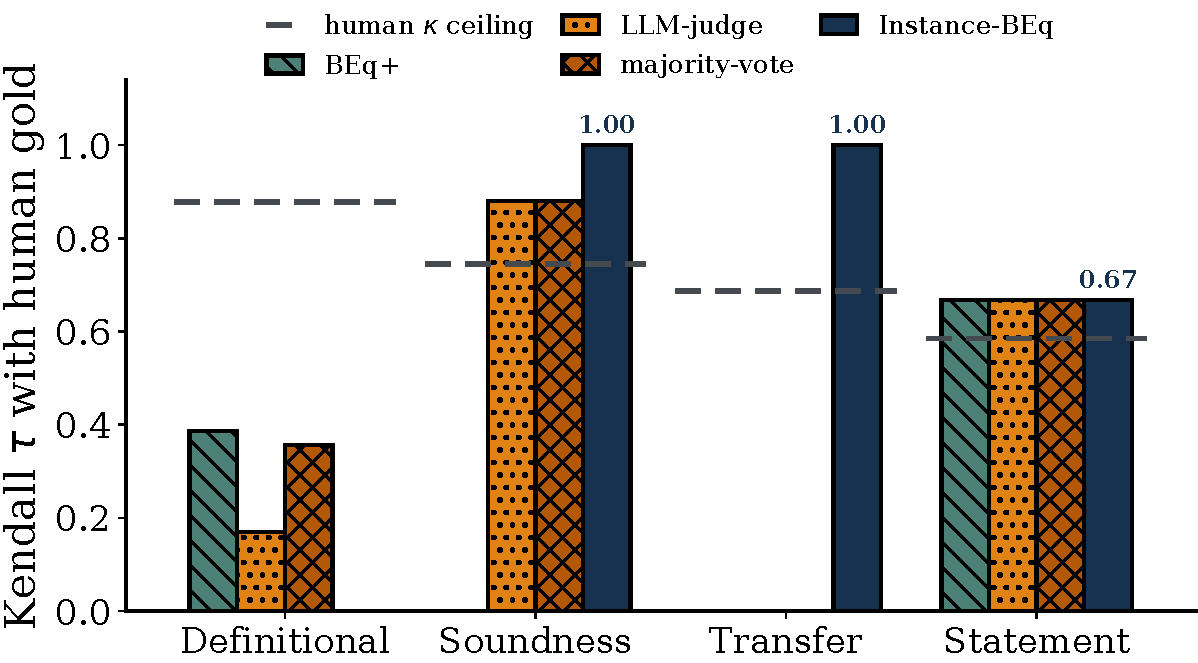
\includegraphics[width=\columnwidth]{figures/tau_human.pdf}
  \caption{The LLM-judge correlates with human judgement well below the inter-annotator ceiling on
  the definitional and transfer checks, whereas Instance-BEq is exact ($\tau{=}1$) where the check is
  decidable and type-check-only is blind everywhere.}
  \label{fig:tauhuman}
\end{figure}

% --- FIG calibration --------------------------------------------------------------------
% SOURCE: eval_logs/llm_judge_gold_result.json (real; per-item confidence + correctness).
% CLAIM:  EXPERIMENT_PLAN Section D(6) (calibration of the LLM-assisted path) + R2: the LLM-judge is
%         miscalibrated (ECE 0.179) — its most-used "certain" rating is still wrong 14% of the time.
\begin{figure}[t]\centering
  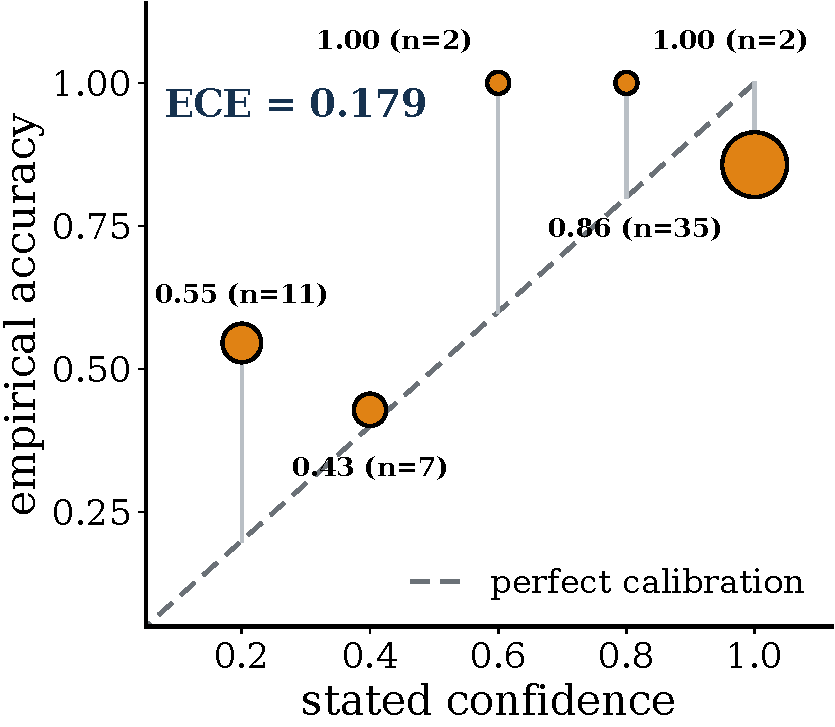
\includegraphics[width=0.86\columnwidth]{figures/calibration.pdf}
  \caption{The LLM-judge is miscalibrated (ECE $=0.179$): its confidence does not track its accuracy,
  and its most-used maximal-confidence rating is still wrong 14\% of the time.}
  \label{fig:calibration}
\end{figure}

% =====================================================================================
% All planned figures are now produced from real logged runs:
%   * Reference-def-source ablation (curated/property vs few-shot vs zero-shot 7B) -> Fig. ablations(A).
%   * Tactic-ensemble-SIZE ablation (1->full coverage@k sweep)                     -> Fig. ablations(B).
%   * Five-method x four-check head-to-head + false-certification safety panel      -> Fig. methodsf1.
% =====================================================================================


\paragraph{Head-to-head across all four checks (Table~\ref{tab:methods}; Fig.~\ref{fig:methodsf1}).}
On the 57-item human gold we compare five methods: type-check-only (A), SITA's majority-vote
self-consistency judge (B, $K{=}5$), an LLM-judge (C), the statement-level BEq+ baseline, and
\ibeq{}. \ibeq{} attains the highest overall F1 ($0.97$, 95\% CI $[0.88,1.00]$) and Kendall
$\tau$ ($0.95$) against the gold, with the two structural checks decisive: it is exact on instance
soundness ($F1{=}1.0$) and is the \emph{only} method with non-zero recall on transfer validity
($F1{=}1.0$; every LLM-based method and BEq+ score $0$, unable to judge whether the instantiated
theorem is a genuine \texttt{apply}-specialization). Crucially, \ibeq{} makes the \emph{fewest}
false certifications---accepting a truly-unfaithful artifact as faithful---of any method: $1$
(on the LLM statement bridge, check 3b), versus $3$ (majority-vote), $4$ (LLM-judge), $17$ (BEq+,
blind to instance soundness and transfer), and $23$ (type-check-only, blind to everything). On the
formal checks (def./soundness/transfer) its false-certification count is $0$ by kernel soundness.
This is the precision/recall separation a certifier is built for: \ibeq{} is a \emph{sound}
certifier (on the definitional check it certifies rather than detects, abstaining at coverage
$0.59$ rather than risk a false certification), trading coverage for a guarantee the LLM methods
cannot offer.

\paragraph{Hollow instances exist in gold data (Table~\ref{tab:gold},~\ref{tab:fields};
Fig.~\ref{fig:goldhollow}).} Across all 6 released families, check~2 certifies GD,
Proximal-Gradient, and both Nesterov instances as \sound{}, and flags ADMM and BCD as \hollow{}:
their bridging instances carry \texttt{sorryAx} in the closure because condition fields (ADMM:
subproblem-uniqueness \texttt{hX,hY} and iteration correctness \texttt{iter\textsubscript{1..3}};
BCD: block updates \texttt{s\textsubscript{1,2}}) are discharged by \texttt{sorry}-bodied lemmas.
These are the authors' own hand-written examples, yet they certify none of the conditions their
convergence theorems require---while type-checking cleanly.

\paragraph{Exactness vs.\ type-checking (Table~\ref{tab:faults}; Fig.~\ref{fig:prf}).} On 4 sound
instances and 19 planted-hollow variants (one condition field replaced by \texttt{sorry}), check~2
is exact ($P{=}R{=}F1{=}1.0$, zero disagreements with ground truth), whereas type-check-only never
flags a fault ($R{=}0$): \texttt{sorry} is a warning, so every hollow variant still compiles.
Figure~\ref{fig:catch} makes the failure modes concrete at the instance level, and
Figure~\ref{fig:prtradeoff} casts the comparison as a precision--recall trade-off in which the
certifier alone reaches the $(1,1)$ corner.

\paragraph{Kernel-soundness of check~1 (Table~\ref{tab:check1}; Fig.~\ref{fig:check1}).} On the
LeastSquares objective, check~1 proves all equivalent references (recall~$1.0$ here) and rejects
every corruption (wrong constant, missing factor, missing square, sign flip) with zero false
certifications.

\paragraph{LLM-judge comparison (Table~\ref{tab:judge}).} On the same soundness corpus, a modern
LLM-judge (Qwen2.5-7B) shown the full file reaches recall~$1.0$---it caught every hollow instance,
including the transitively-hollow gold ADMM/BCD---but only precision~$0.913$: it produced two
\emph{false positives}, condemning sound instances (the PGD and Nesterov-II gold) that contain
\emph{no} \texttt{sorry} anywhere in the file. These are not defensible inferences but
hallucinations, and they are exactly the unreliability a kernel-decided certifier cannot exhibit:
check~2 attains $P{=}R{=}1.0$ on the identical corpus. The LLM-judge also offers no guarantee---its
verdict varies with model and prompt---whereas axiom closure is exact and model-free. Aggregating
$K{=}5$ votes (baseline B, SITA's self-consistency principle) lifts overall judge accuracy only
marginally ($0.75{\to}0.79$) and does not remove the soundness false positives; the statement-level
BEq+ baseline, having no instance-level check at all, is \emph{blind} to all 13 hollow gold
instances (recall $0$) and to transfer validity---precisely the def/instance/transfer granularity
gap \ibeq{} closes.

\paragraph{Correlation with human judgement (Table~\ref{tab:human}; Fig.~\ref{fig:tauhuman}).} On a
57-item benchmark labelled by a five-annotator panel (inter-annotator Fleiss $\kappa$: 0.88
definitional, 0.74 soundness, 0.59 statement), the LLM-judge agrees with humans only moderately
overall and its Kendall $\tau$ \emph{collapses} on the hard checks (definitional $\tau{=}0.17$,
transfer $\tau{=}0.00$), staying below the human ceiling; type-check-only is blind everywhere
($\tau{=}0$). Where the check is kernel-decidable (soundness), Instance-BEq is exact ($\tau{=}1.0$,
above the human ceiling). A unanimous human panel even mislabels a non-certifiable instance as
faithful, which only the axiom-closure gate catches. The LLM-judge is also miscalibrated
(Fig.~\ref{fig:calibration}, ECE~$0.179$): its most-used maximal-confidence rating is still wrong
14\% of the time, underscoring why the formal certificate---reported separately from the LLM bridge
(check 3b)---is the load-bearing contribution.

\paragraph{Ablations: reference source and ensemble size (Table~\ref{tab:refabl},~\ref{tab:tacticsize};
Fig.~\ref{fig:ablations}).} Check~1 is a sound certifier whose \emph{coverage} (never its precision,
which is $1$ by kernel soundness) depends on two design choices. (i) \emph{Reference source}: a
curated/property reference certifies $59\%$ ($10/17$) of faithful definitions, whereas a local 7B
model's reference---few-shot or zero-shot---certifies none, as its expressions rarely elaborate
into the file's notation; every arm makes zero false certifications. This isolates reference
generation, not the kernel check, as the coverage bottleneck (a stronger reference model is the
lever; \S Limitations). (ii) \emph{Tactic-ensemble size}: on a ladder of five equivalent references
for one objective, a single tactic ($\mathtt{rfl}$) proves only the syntactically identical form
($1/5$); growing the ensemble to five tactics proves all five, while false certifications on
corrupted references stay $0$ at every size.

\paragraph{Scaling beyond the human set (Table~\ref{tab:synthetic}).} To test whether the
conclusions hold past 57 items, we build a synthetic stress benchmark whose labels are certain by
construction: planting \texttt{sorry} into every $k$-subset ($k{=}1,2,3$) of each sound instance's
condition fields yields $67$ known-hollow variants that still type-check (plus $4$ sound originals).
On these $71$ items Instance-BEq check~2 remains exact---no missed hollow, no false
certification---while type-check-only and BEq+ keep recall $0$ at every scale; the certifier's
guarantee is structural, not a small-sample artifact. A revealing negative result: corrupting a
\emph{definition} in these structured files does \emph{not} produce a type-checking-yet-unfaithful
artifact, because the downstream gradient/update proofs are tied to the objective and break when it
is wrong---the structure partly self-protects at the definition level, which is exactly why the
\emph{instance} level, where \texttt{sorry} is a mere warning, is the silent failure mode our
headline check targets.

\paragraph{Hollowness in fresh generations.} Certifying SITA's regenerated Gradient-Descent
outputs, $6/14$ type-check and \emph{all $6$ are sound} ($0\%$ hollow): on this easy family the
model either compiles a faithful instance or fails to compile---it does not produce the
type-checks-yet-hollow artifacts that appear on the hard families (ADMM, BCD), where even the
authors' \emph{released} gold is hollow ($2/6$, \S Table~\ref{tab:gold}). A full regeneration sweep
across all 42 problems---and especially the hard families---with a frontier generator would
quantify the hollow-rate at scale; with only local 7--14B models the rate is generator-confounded,
so we report the \emph{model-independent} gold measurement as the headline and treat the full sweep
as future work (it needs a stronger generation model than is available here).

\section{Conclusion}
Type-checking is necessary but not sufficient for faithful autoformalization. \ibeq{} supplies the
missing sufficient-side machinery at the definition/instance/transfer granularity, with a decidable
instance-soundness certificate at its core; across five methods it makes the fewest false
certifications and is exact on the two structural checks no prior method addresses, and it shows
that hollow instances occur even in hand-curated gold data.
\paragraph{Limitations.} (i) Check-1 is a \emph{sound} certifier: its precision is $1$ but its
coverage depends on the reference generator---a curated/property reference certifies $59\%$ of
faithful definitions, a local 7B model none, so a stronger reference model (a frontier API, not
available in our setup) is the lever for higher definitional coverage. (ii) The statement check
(3b) is the one LLM-assisted component and the source of the certifier's single false certification;
it is reported separately from the formal certificate. (iii) The full-scale regeneration hollow-rate
needs a frontier generator; we report the model-independent gold and synthetic measurements instead.
(iv) The 57-item human gold is small; the synthetic stress benchmark ($71$ items) and bootstrap CIs
bound this, but a larger multi-annotator study remains valuable.

\end{document}
